% qsvm.tex

Given training data embedded as n-qubit quantum states \(\{\ket*{x_i}\}\) with
corresponding labels \({y_i = \pm 1}\), a QSVM implemented as a VQA attempts to learn a
unitary \(\pqc(\parameters)\) such that

\begin{equation}
    \text{sgn }{\ket*{0}^{\otimes n}\pqc(\parameters)^*\ket*{x_i}} = y_i \forall i~.
\end{equation}

Setting \(\ket*{w} = \pqc(\parameters)\ket*{0}^{\otimes n}\) recovers the
familiar classical SVM from \autoref{eq:svmclassifier}.

An \(\epsilon\) error in the unitary correspondingly generates an error in
\(\ket*{w}\) and generates a conical section (more generally, a hypersector of
an n-hypersphere) as seen in \autoref{fig:qsvmerrorcone}.

\begin{figure}[!ht]
    % error cones
    \centering
    \begin{tikzpicture}[>=stealth']
        % Draw axes
        \draw [<->,thick] (0,5) node (yaxis) [above] {}
              |- (5,0) node (xaxis) [right] {};
        \draw [<->,thick] (0,-5) node (negyaxis) [above] {}
              |- (-5,0) node (negxaxis) [right] {};
        % classifier
        \draw[red, thick] (-4, -4) -- (4, 4);
        \draw[red, thick,->] (0, 0) -- node[very near end, right] {\(~\ket*{w}\)} (+1, -1);
        % error bars
        \draw (-3.5, -4.5) -- (3.5, 4.5) [dashed];
        \draw[->] (0, 0) -- (1.2, -0.8)[dashed];
        \draw (-4.5, -3.5) -- (4.5, 3.5) [dashed];
        \draw[->] (0, 0) -- node[very near end, below] {\(\ket*{w_\epsilon}\)} (0.8, -1.2)[dashed];
      \end{tikzpicture}
      \caption{Intuitive representation of error in the hyperplane normal vector.}
      \label{fig:qsvmerrorcone}
\end{figure}

Picking a point randomly in the space outside the training data and attempting
to classify it, we find an error probability proportional to the volume of the
hypersector generated by the error in \(\ket*{w}\). We have using volume
formulae from \cite{li2011concise}

\begin{align}
        p_{\text{error}} &= \lim_{r\to \infty}\frac{2\cdot V_{\text{sector}}(r)}{V_{\text{sphere}}(r)} \nonumber\\
            &= \lim_{r\to \infty}\frac{2\cdot V_{\text{sphere}}(r)\cdot 0.5\cdot I_{\text{sin}^2\phi}(\frac{n-1}{2}, \frac{1}{2})}{V_{\text{sphere}}(r)} \nonumber\\
            &= I_{\text{sin}^2\phi}(\frac{n-1}{2}, \frac{1}{2})~,
\end{align}

where \(I\) is the incomplete Beta function, 

\begin{equation}
    I_x(a, b) = \frac{B(x; a, b)}{B(a, b)} = \frac{\int_0^x t^{a-1} (1-t)^{b-1} \dd t}{\int_0^1 t^{a-1} (1-t)^{b-1} \dd t}~,
\end{equation}

and \(\phi\) is the angular distortion, and it is seen from \(\ket*{w} =
\pqc(\parameters)\ket*{0}\) that \(\text{sin} \phi \sim \epsilon\). Finally, we
have,

\begin{equation}
    p_{\text{error}} \sim I_{\epsilon^2}(\frac{n-1}{2}, \frac{1}{2})~.
\end{equation}

For a fixed \(\epsilon\), this error probability falls off quite quickly with
\(n\). See \autoref{fig:perrorplot} for plots of the probability with varying
\(n\) at different values of \(\epsilon\). The form of the function suggests
that while there is a fundamental limit to learning the unitaries, it may not
always be a hindrance to be wary of, provided the system is of sufficiently
high dimension.

\begin{figure}
    \centering
    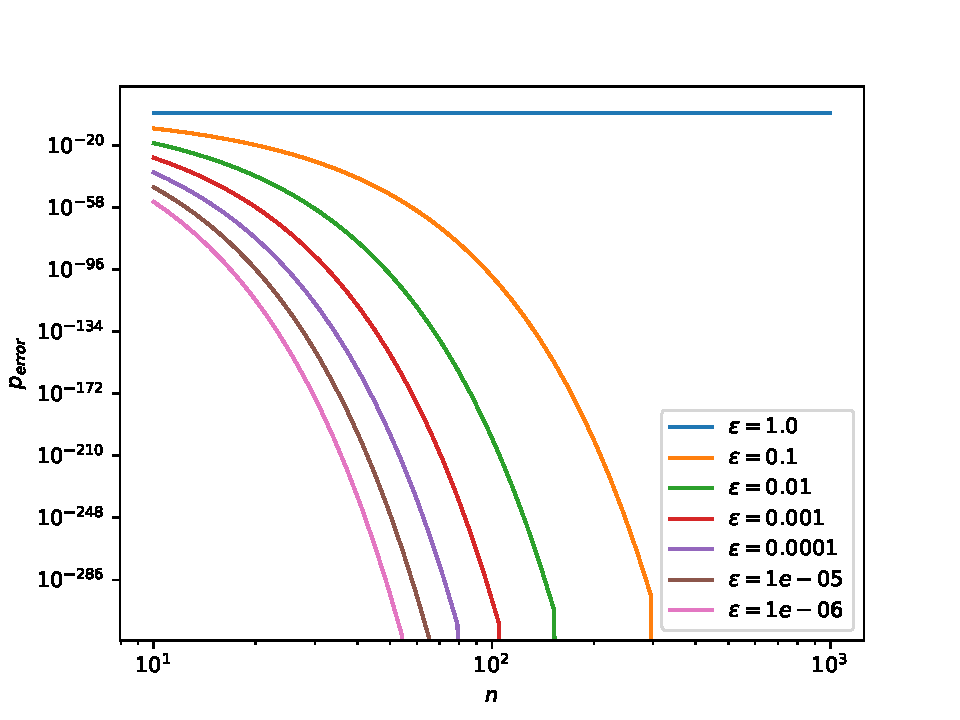
\includegraphics[width=0.8\textwidth]{figures/perrorplot.pdf}
    \caption{\(p_{\text{error}}\) with change in \(n\) at several values of \(\epsilon\).}
    \label{fig:perrorplot}
\end{figure}

However, it is to be noted that this analysis uses a fixed value of the unitary
distortion, \(\epsilon\). In a real system, this is certainly not expected to be
independent of the circuit width (number of qubits, dimension of state space).
Preliminary calculations as described in \autoref{sec:infolimits} suggest that
\(\epsilon\) is a function of the circuit area, i.e., the circuit width and
depth product. This is related to the quantity \(M\) described in
\autoref{subsubsec:pqc}. So, an increase in width correspondingly leads to a
\emph{decrease} in depth of the circuit to maintain the same error bounds for
the unitary output.

The depth of the circuit has been heavily correlated to the barren plateau
problem \cite{larocca2021theory}. Increasing the depth of the circuit has been
identified to remove spurious minimas from the problem and overparametrization
beyond a certain depth (characterized by the QFIM) leads to deepening of present
minimas, with a tradeoff towards barren plateaus \cite{larocca2021diagnosing}.
This new result presents a second tradeoff. If we keep the error constant, and
thus by the hypothesis, the area, the reduction in error by increase in width
(upto a certain level, see \autoref{fig:perrorplot}) would require a decrease in
depth, leading to spurious minimas. This tradeoff is a subject of our current
study.

\begin{figure}[ht]
    \centering
    %
    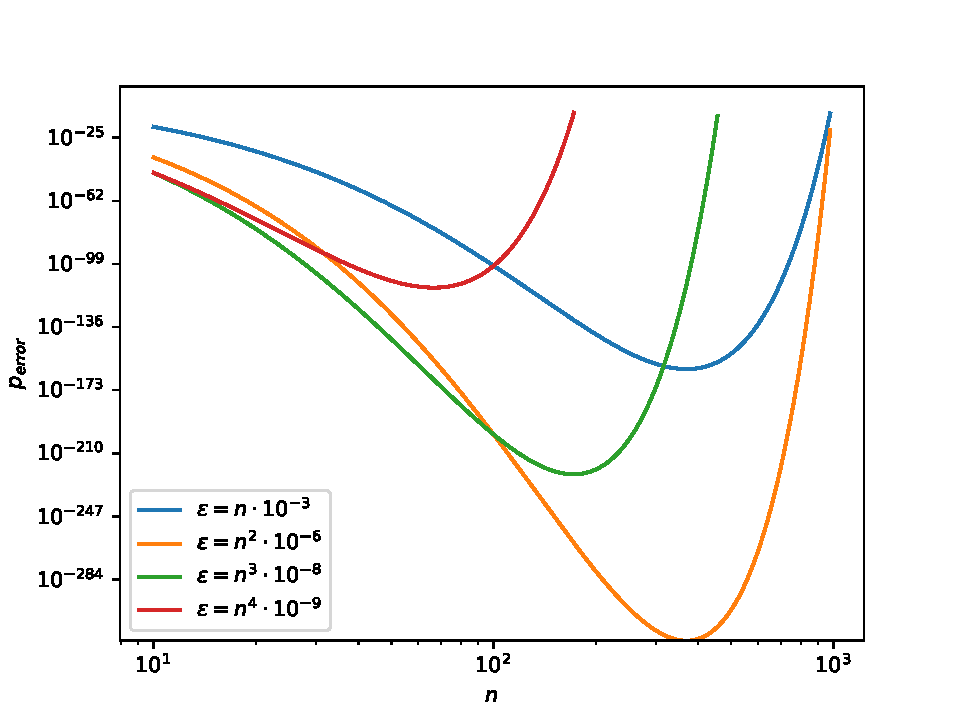
\includegraphics[width=0.8\textwidth]{figures/perrorscaled.pdf}
    \caption{\(p_{\text{error}}\) scaling assuming \(\epsilon\) changes with \(n\).}
    \label{fig:perrorscaled}
\end{figure}

For illustration, values of the error probability are plotted in
\autoref{fig:perrorscaled} with different scaling functions chosen for
\(\epsilon\) dependent on n, assuming a fixed circuit depth. Note that scaling
higher than linear would lead to an optimal width to perform learning problems
at, provided the depth is fixed, where the generalization error is expected to
be minimum. The exact scaling form is not currently known.
